\documentclass[10pt]{beamer}
\usetheme[
%%% option passed to the outer theme
%    progressstyle=fixedCircCnt,   % fixedCircCnt, movingCircCnt (moving is deault)
  ]{Feather}
  
% If you want to change the colors of the various elements in the theme, edit and uncomment the following lines

% Change the bar colors:
%\setbeamercolor{Feather}{fg=red!20,bg=red}

% Change the color of the structural elements:
%\setbeamercolor{structure}{fg=red}

% Change the frame title text color:
%\setbeamercolor{frametitle}{fg=blue}

% Change the normal text color background:
%\setbeamercolor{normal text}{fg=black,bg=gray!10}

%-------------------------------------------------------
% INCLUDE PACKAGES
%-------------------------------------------------------

\usepackage[utf8]{inputenc}
\usepackage[english]{babel}
\usepackage[T1]{fontenc}
\usepackage{helvet}

%-------------------------------------------------------
% DEFFINING AND REDEFINING COMMANDS
%-------------------------------------------------------

% colored hyperlinks
\newcommand{\chref}[2]{
  \href{#1}{{\usebeamercolor[bg]{Feather}#2}}
}

%-------------------------------------------------------
% INFORMATION IN THE TITLE PAGE
%-------------------------------------------------------

\title[] % [] is optional - is placed on the bottom of the sidebar on every slide
{ % is placed on the title page
      \textbf{Hidden Markov Models}
}

\subtitle[Hidden Markov Models]
{
      \textbf{v. 1.0.0}
}

\author[Tien Anh Nguyen]
{      Tien Anh Nguyen \\
      {\ttfamily tien.nguyenanh94@gmail.com}
}

\institute[]
{
      Faculty of Electronics and Computer Engineering\\
      Chonnam National University\\
  
  %there must be an empty line above this line - otherwise some unwanted space is added between the university and the country (I do not know why;( )
}

\date{\today}

%-------------------------------------------------------
% THE BODY OF THE PRESENTATION
%-------------------------------------------------------

\begin{document}

%-------------------------------------------------------
% THE TITLEPAGE
%-------------------------------------------------------

{\1% % this is the name of the PDF file for the background
\begin{frame}[plain,noframenumbering] % the plain option removes the header from the title page, noframenumbering removes the numbering of this frame only
  \titlepage % call the title page information from above
\end{frame}}


\begin{frame}{Content}{}
\tableofcontents
\end{frame}

%-------------------------------------------------------
\section{References}
%-------------------------------------------------------
\begin{frame}[allowframebreaks]{References}
%-------------------------------------------------------
\begin{thebibliography}{9}
 \bibitem {Richard} Richard A. Davis
  \newblock Introduction to Statistical Analysis of Time Series.
 \bibitem {Brian} Prof. Brian Charles Williams \& Prof. Emillio Frazzoli
  \newblock Principles of Autonomy and Decision Making course.
  \newblock \emph{MIT OpenCourseWare} 16.410/413, Lecture 20
 \bibitem {Dimitri} Dimitri P. Bertsekas \& John N. Tsitsiklis
  \newblock Introduction to Probability, 2002
  \newblock Massachusetts Institute of Technology
  \newblock Department of Electrical Engineering and Computer Science
 \bibitem {Thomas} Thomas Mailund
  \newblock Pattern Recognition In BioInformatics Q3/2012
  \newblock Aarhus University
  \newblock Department of Computer Science
 \bibitem {Anders} Anders Meng
  \newblock An introduction to Markov and Hidden Markov Models
 \bibitem {Daniel} Daniel Ramage
  \newblock Machine Learning CS229
  \newblock Stanford University
  \newblock December 1, 2007
 \bibitem {UDACITY} Aaron Bobick \& Irfan Essa \& Arpan Chakraborty 
  \newblock Introduction to Computer Vision
  \newblock UDACITY
  \newblock \emph{https://www.udacity.com/course/ud810}
\end{thebibliography}
\end{frame}

%-------------------------------------------------------
\section{Big Picture}
%-------------------------------------------------------
\subsection{Time Series}
\begin{frame}{Big Picture}{Time Series}
%-------------------------------------------------------
  \begin{itemize}
    \item Time Series: A collection of observations $x_t$ each one being \
          recorded at time t. (Time could be discrete, t = 1, 2, 3, ..., or \
          continuous t > 0). \cite{Richard}
  \end{itemize}
\end{frame}

%-------------------------------------------------------
\subsection{Whey do we need Markov and Hidden Markov Models?}
%-------------------------------------------------------
\begin{frame}{Big Picture}{iid}
%-------------------------------------------------------
  \begin{itemize}
    \item A model is that observations are assumed to be independent \
          and identically distributed (iid). \cite{Thomas}
  \end{itemize}
  \begin{figure}[h]
    \centering
    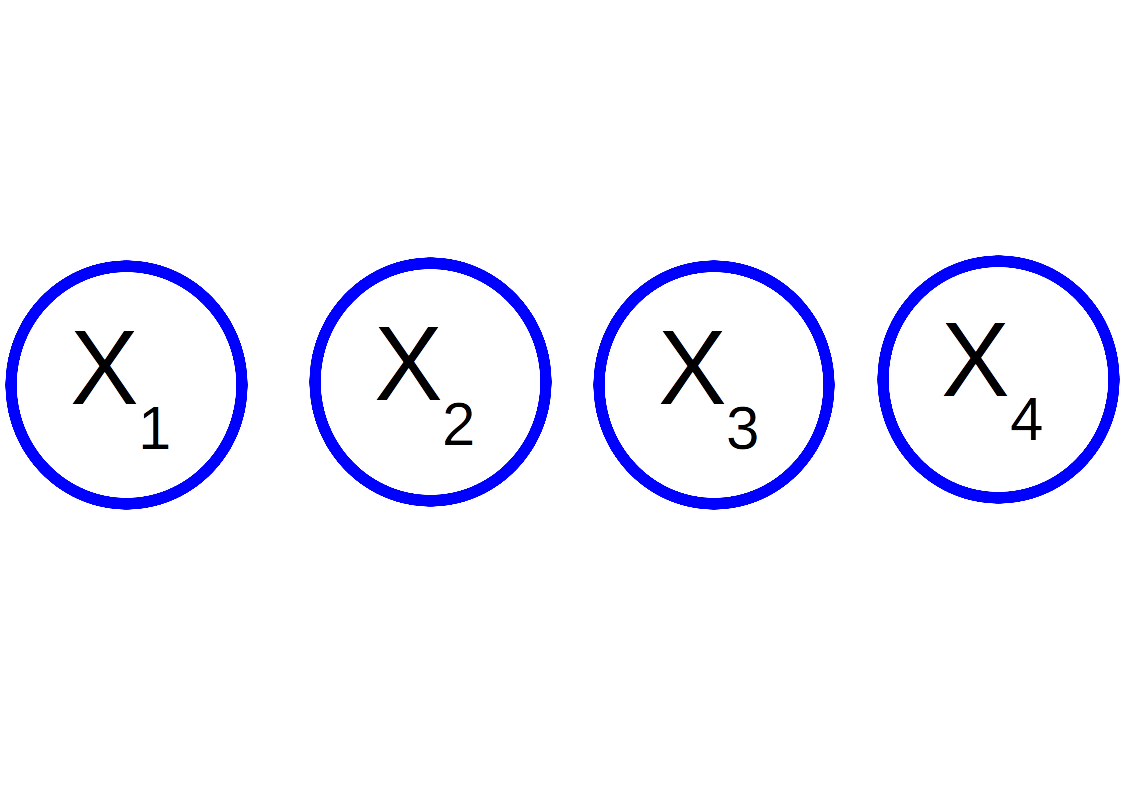
\includegraphics[width=2in,height=2in]{figures/idd.png}
  \end{figure}
\end{frame}

%-------------------------------------------------------
\begin{frame}{Big Picture}{Whey do we need Markov and Hidden Markov Models?}
%-------------------------------------------------------
  \begin{itemize}
    \item What are going to happend if observation are dependent?
    \item How can we calculate the "likelihood" of the sample?
  \end{itemize}
  \begin{figure}[h]
    \centering
    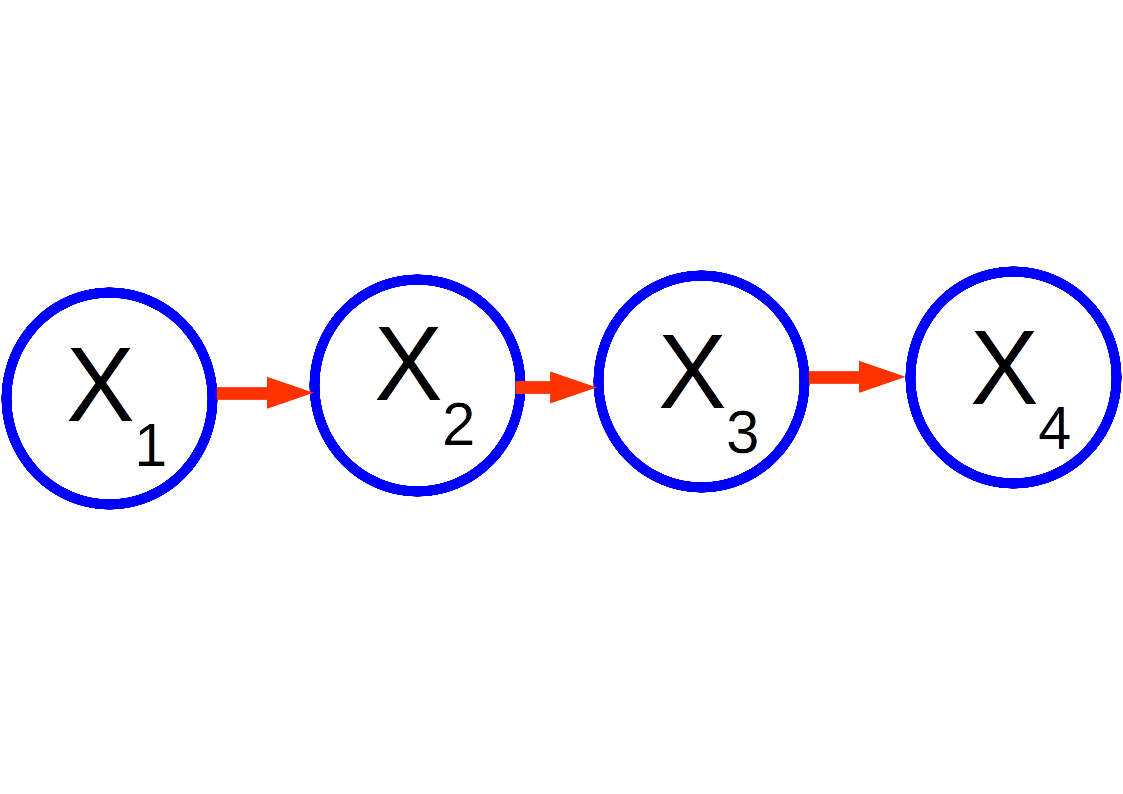
\includegraphics[width=2in,height=2in]{figures/not_idd.png}
  \end{figure}
\end{frame}

\begin{frame}{Big Picture}{Whey do we need Markov and Hidden Markov Models?}
%-------------------------------------------------------
  \begin{itemize}
    \item How can we predict weather of next day based on weather of today?
  \end{itemize}
  \begin{figure}[h]
    \centering
    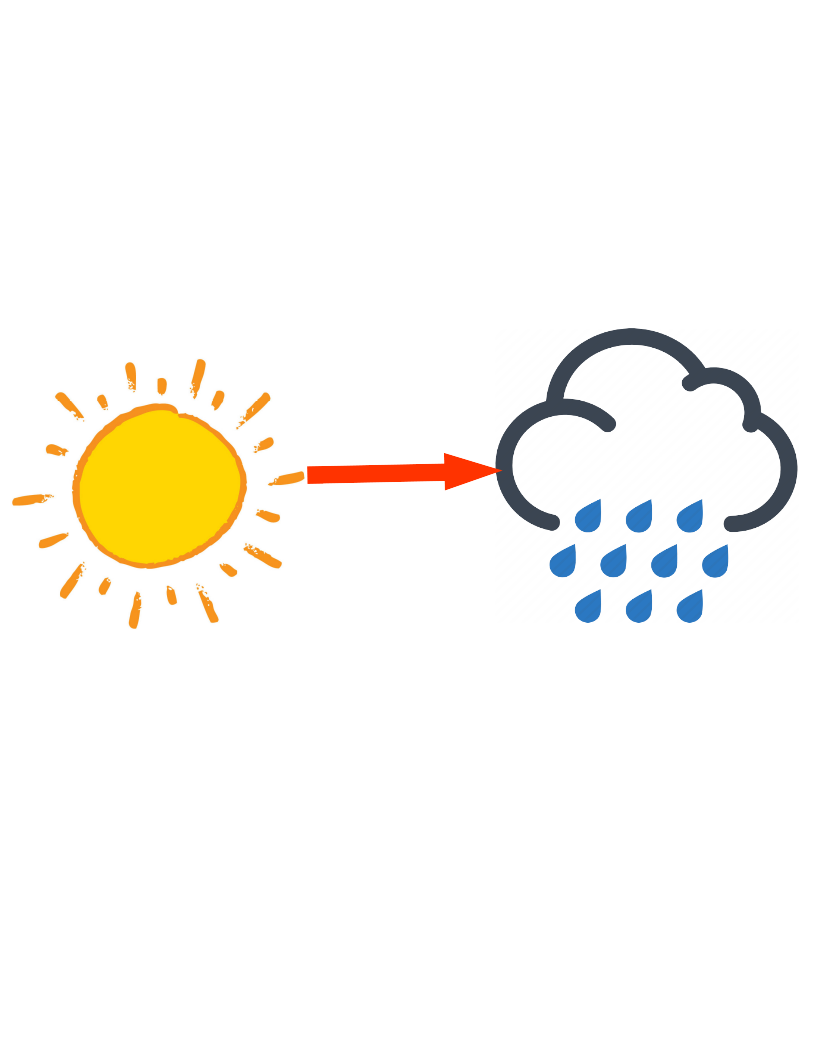
\includegraphics[width=1in,height=1in]{figures/sunny_to_rainny.png}
  \end{figure}
\end{frame}
%-------------------------------------------------------------------------

\begin{frame}{Big Picture}{Whey do we need Markov and Hidden Markov Models?}
%-------------------------------------------------------
  \begin{itemize}
    \item How can we predict weather of next day based on weather of today?
  \end{itemize}
  \begin{figure}[h]
    \centering
    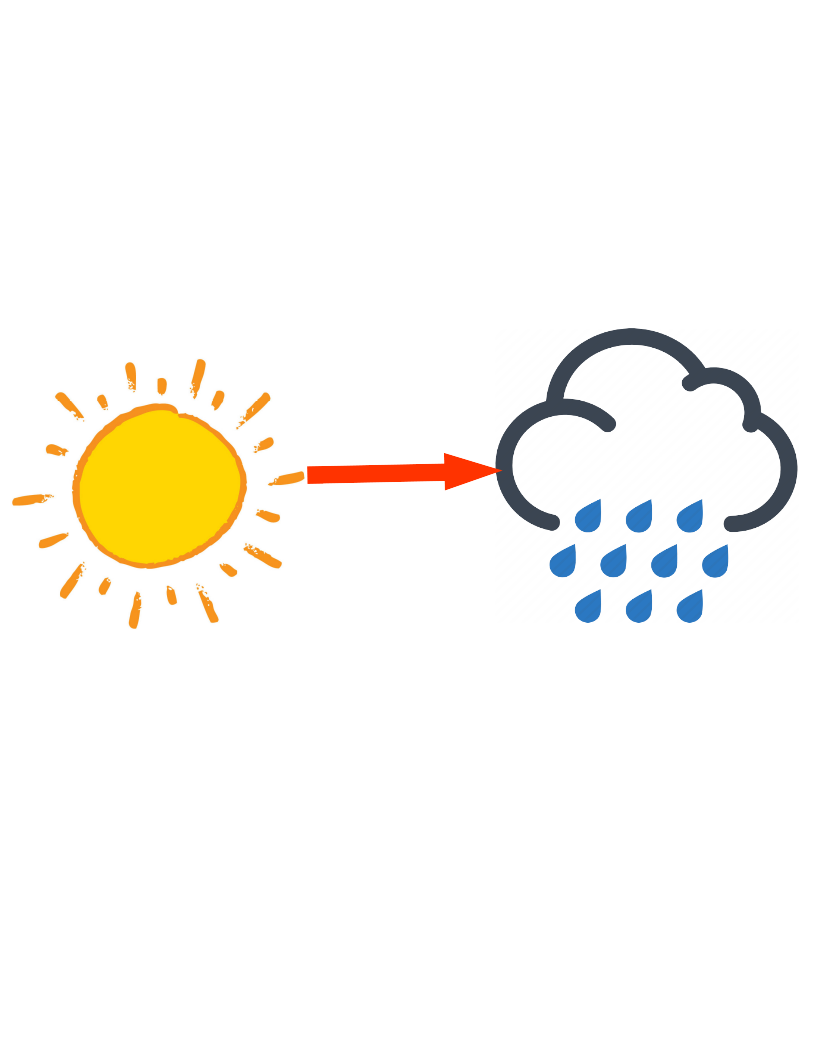
\includegraphics[width=1in,height=1in]{figures/sunny_to_rainny.png}
  \end{figure}
\end{frame}

\begin{frame}{Big Picture}{Whey do we need Markov and Hidden Markov Models?}
%-------------------------------------------------------
  \begin{itemize}
    \item Assume that you have been locked into a room for serveral days, \
          and you have no windows, so can we predict the weather outside \
          based on the clothes of the caretaker?
  \end{itemize}
  \begin{figure}[h]
    \centering
    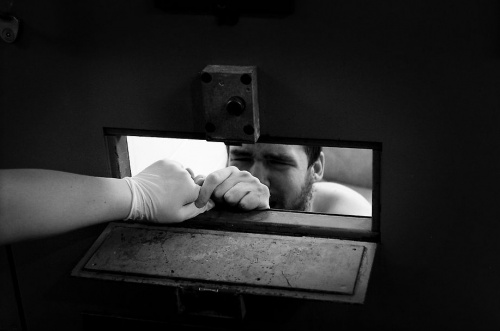
\includegraphics[width=3in,height=2in]{figures/prisoner.jpg}
  \end{figure}
\end{frame}
%-------------------------------------------------------

%-------------------------------------------------------
\section{Markov Chain}
%-------------------------------------------------------
\subsection{Ingredients of a Markov Chain}
\begin{frame}{Markov Chain}{Ingredients}
  \begin{itemize}
    \item States: ${S_1, S_2, ..., S_N}$ 
    \item States transition probabilities: 
                          $a_{ij} = P(z_{t+1} = S_i | z_t = S_j)$ 
    \item Initial state distribution: $\pi_{i} = P(z_1 = S_i)$ 
  \end{itemize}
\end{frame}
%-------------------------------------------------------

%-------------------------------------------------------
\begin{frame}{Markov Chain}{Example 1}
%-------------------------------------------------------
  \begin{block}{Example 1}
     We have 3 states from a weather system $S = {Sunny, Rainy, Snowy}$
  \end{block}
\end{frame}
%-------------------------------------------------------

%-------------------------------------------------------
\subsection{Markov Assumption}
\begin{frame}{Markov Chain}{Markov Assumption}
%-------------------------------------------------------
  \begin{block}{LIMITED HORIZON ASSUPTION}
        The probability of being in a state at time $t+1$ depends only on the\
        state at time $t$. It means that the state at time $t$ represents\
        "enough" summary of the past to reasonably predict the feature. Formally:
  \end{block}
\end{frame}
%-------------------------------------------------------

%-------------------------------------------------------
\subsection{Definition}
\begin{frame}{Markov Chain}{DEFINITION}
%-------------------------------------------------------
  \begin{block}{Definition(Markov Chain)}
     A Markov chain is a sequence of random variables \ 
     $X_1,\ X_2,\ X_3,\ ...,\ X_t,\ ...$, such that the probability\
     distribution of $X_{t+1}$ depends only on t and $x_t$. \cite{Brian}
  \end{block}
  In other words:
       $P(X_{t+1} = x | X_t = x_t, \textcolor{red}{X_{t-1} = x_{t-1}, ..., X_1 = x_1}) = P(X_{t+1} = x|X_t = x_t)$
\end{frame}

%-------------------------------------------------------
{\1
\begin{frame}[plain,noframenumbering]
  \finalpage{Thanks for your attention}
\end{frame}}

\end{document}
